%%%%%%%%%%%%%%%%%%%%%%%%%%%%%%%%%%%%%%%%%%%%%%%%%%%%%%%%%%%%%%%
% P3b MLP
% David Miguel Lozano
% Javier Martínez Riberas
% Universidad de Burgos - Noviembre 2016
%%%%%%%%%%%%%%%%%%%%%%%%%%%%%%%%%%%%%%%%%%%%%%%%%%%%%%%%%%%%%%%

% -------------------------------------------------------------
% Preamble
% -------------------------------------------------------------
\documentclass[a4paper,12pt,titlepage]{article}

% -------------------------------------------------------------
% Packages
% -------------------------------------------------------------
\usepackage[utf8]{inputenc}	% Unicode support
\usepackage[T1]{fontenc}		% Font encoding
\usepackage[spanish]{babel}	% Languaje
\usepackage{lmodern}	% Typeface 
\usepackage{textcomp} % Special symbols
\usepackage{graphicx}	% Add pictures
\usepackage{pgfplots} % Graphs and charts
\usepackage{hyperref}	% Add a link to index entries
\usepackage{amsmath}	% Advanced math typesetting
\usepackage{amsfonts}	% Mathematical formulas
\usepackage{amssymb}	% Extended symbol collection
\usepackage{listings}	% Code formatting and highlighting
\usepackage{xcolor}		% Color package
\usepackage{enumitem}	% Customizing lists
\usepackage{parskip}	% Paragraph styles
\usepackage[a4paper]{geometry} 		% Margins
\usepackage[numbers,sort]{natbib}	% Bibliography management
\usepackage{booktabs}							% Tables

% -------------------------------------------------------------
% Configuration
% -------------------------------------------------------------
% Images path
\graphicspath{ {img/} }
% Graphs configuration 
\pgfplotsset{width=\textwidth,compat=1.9}
% Hyperlinks coloring
\hypersetup{
	colorlinks,
	linkcolor={green!40!black},
	citecolor={blue!50!black},
	urlcolor={blue!80!black}
}
% Define HRule
\newcommand{\HRule}[1]{\rule{\linewidth}{#1}}
% Define listings styles
\definecolor{codebg}{HTML}{EEEEEE}
\definecolor{codeframe}{HTML}{CCCCCC}
\definecolor{comments}{HTML}{009900}
\lstset{
  language=Matlab, 								% Programming language 
  backgroundcolor=\color{codebg},	% Background color
  frame=single, 									% Add frame around code
	framesep=10pt,									% Padding
	rulecolor=\color{codeframe},		% Don't change frame color
	upquote=true,										%
	breakatwhitespace=true,					% Break line only in spaces
	keepspaces=true,								% Keep indentation
	tabsize=2,											% Tab size
	title=\lstname, 								% Show filename as caption
	basicstyle=\ttfamily, 					% Size and font
  keywordstyle=\color{black}\ttfamily,
	commentstyle=\color{comments},	% Color of comments
  morecomment=[l][\color{magenta}]{\#}
}
% Define style table
\setlength{\heavyrulewidth}{1.5pt}
\setlength{\abovetopsep}{4pt}
\begin{document}
% -------------------------------------------------------------
% Cover
% -------------------------------------------------------------
\author{David Miguel Lozano \ Javier Martínez Riberas}
\title{P3 Multilayer Perceptron (MLP)}
\date{07-11-2016}

\begin{titlepage}
	\centering
	
\includegraphics[width=0.16\textwidth]{ubu-logo.png}\par
	\vspace{0.3cm}
	{\scshape\LARGE Universidad de Burgos \par}
	\vfill
	{\scshape\Large Computación Neuronal y Evolutiva \par}
	\HRule{2pt}
	{\huge\bfseries P3: Multilayer Perceptron (MLP) \par}
	\HRule{2pt}
	\\ [0.5cm]
	{Diseñar y entrenar distintos Perceptrón Multicapa (MLP), con el objetivo de hacer una comparativa respecto al rendimiento de estos para la misma tarea y aplicación estudiada en P1\_Thyroid.}
	\vfill
	Estudiantes:\par
	{\Large\scshape David Miguel Lozano \\ Javier Martínez Riberas \par}
	\vfill
	Profesor de la asignatura:\par
	\textsc{Álvaro Herrero Cosío}
	\vfill
	{\large 1º semestre 2016 \par}
\end{titlepage}

% -------------------------------------------------------------
% Contents
% -------------------------------------------------------------
\newpage
\tableofcontents
\begin{appendix}
  %\listoffigures
  %\listoftables
\end{appendix}

% -------------------------------------------------------------
% Body
% -------------------------------------------------------------
\newpage

\section{Introduction}

El objetivo de la práctica es diseñar y entrenar distintos Perceptrón Multicapa (MLP), con el objetivo de hacer una comparativa respecto al rendimiento de estos para la misma tarea y aplicación estudiada en \href{https://github.com/davidmigloz/neuronal-networks/tree/master/P1\_Thyroid}{P1\_Thyroid} (clasificación de patrones: tiroides).

Se realizará un estudio sobre los distintos algoritmos de aprendizaje que implementan \textit{backpropagation} y el ajuste de los correspondientes parámetros de estos. En concreto:

\begin{itemize}[noitemsep]
	\item \lstinline|net.trainParam.max_fail|: máximo número de fallos de validación.
	\item \lstinline|net.trainParam.alpha|: \textit{learning rate} de los pesos.
	\item \lstinline|net.trainParam.beta|: \textit{learning rate} de los bias.
\end{itemize}

\textit{*En el estudio se explicará porque se han seleccionado estos parámetros para realizar el estudio y no todos los propuestos en el enunciado de la práctica.}

La topología de la red se corresponderá con la configuración más óptima encontrada en la práctica P1\_Thyroid.

\section{Descripción del conjunto de datos}

El conjunto de datos utilizados se ha obtenido del dataset de ejemplo \emph{Thyroid} que provee Matlab. Los datos provienen del \emph{UCI Machine Learning Repository} \citep{Asuncion+Newman:2007} y fueron donados por la Universidad de California.

El dataset contiene datos de 7200 pacientes agrupados en dos matrices:

\begin{itemize}[noitemsep]
	\item $thyroidInputs$: matriz de 21x7200 con los datos de los 7200 pacientes caracterizados por 15 atributos binarios y 6 atributos continuos.
	\item $thyroidTargets$: matriz de 3x7200 en donde se asocia un vector de tres clases a cada paciente. En este vector se define a cuál de las tres clases pertenece el paciente.
\end{itemize}

Las tres clases que contiene el dataset son:

\begin{enumerate}[noitemsep]
	\item Paciente sano.
	\item Paciente con hipertiroidismo.
	\item Paciente con hipotiroidismo.
\end{enumerate}

\section{Descripción del procedimiento}

Para automatizar el estudio lo máximo posible, se ha realizado un script que realiza varios entrenamientos con los diferentes algoritmos de entrenamiento y variando los parámetros mencionados. 

Por cada combinación se ejecutan 20 experimentos y se toma el valor medio para reducir el impacto de la aleatoriedad en la inicialización de los pesos y los bias.

Se han utilizado los siguientes algoritmos de entrenamiento:

\begin{itemize}[noitemsep]
	\item \lstinline|traincgb|: \textit{conjugate gradient backpropagation with Powell-Beale restarts}. \citep{matlab:traincgb}
	\item \lstinline|traincgf|: \textit{conjugate gradient backpropagation with Fletcher-Reeves updates}. \citep{matlab:traincgf}
\end{itemize}

Como se puede observar ambos utilizan el algoritmo de retropropagación para la actualización de los pesos. Y por lo tanto, son adecuados para el entrenamiento de un perceptrón multicapa.

Se modifican los siguientes parámetros para cada algoritmo:

\begin{itemize}[noitemsep]
	\item \lstinline|net.trainParam.max_fail|: \textit{maximum validation failures}. Rango [10:10:100].
	\item \lstinline|net.trainParam.alpha|: \textit{scale factor that determines sufficient reduction in performance}. Rango [0.001:0.001:0.004].
	\item \lstinline|net.trainParam.beta|: \textit{scale factor that determines sufficient large step size}. Rango [0.1:0.2:0.8].
\end{itemize}

Como indicadores generales se han empleado:

\begin{itemize}[noitemsep]
	\item \lstinline|C|: \textit{confusion value (fraction of samples misclassified)}.
	\item \lstinline|plotperform|: \textit{plot network performance}. \citep{matlab:plotperform}
\end{itemize}

\emph{*Todo el código generado en esta práctica se encuentra disponible en el siguiente repositorio: 
\href{https://github.com/davidmigloz/neuronal-networks/tree/master/P3b\_MLP/}{P3b\_MLP}.}

\section{Estudio}

En primer lugar, se han utilizado los parámetros descritos en la sección anterior para realizar el estudio y no todos los propuestos en el enunciado de la práctica (\textit{epochs}, \lstinline|goal| y tiempo de aprendizaje) porque, debido a la experiencia obtenida durante la realización de la práctica 1, somos conscientes que los parámetros elegidos son los más relevantes para este problema en concreto y, por tanto, los más interesantes de estudiar.

Todos los datos generados durante los 320 experimentos del estudio (archivos CSV con los datos recogidos, imágenes con las gráficas de rendimiento y tablas Excel de resumen) se encuentran en el directorio del repositorio: \href{https://github.com/davidmigloz/neuronal-networks/tree/master/P3b\_MLP/data}{Data}. No se incluyen en el informe por no aumentar demasiado la longitud de este.

Tras analizar los datos obtenidos, hemos seleccionado el mejor caso para cada algoritmo y cada parámetro basándonos en el que tuviese el menor valor de confusión medio.

Mejor caso para el algoritmo \lstinline|traincgb|:

\begin{itemize}[noitemsep]
	\item \lstinline|max_fail|: 50.
	\item \lstinline|alpha|: 0.001.
	\item \lstinline|beta|: 0.1.
\end{itemize}

Su gráfico de rendimiento fue:

\begin{figure}[!ht]
	\centering
	\label{fig:traincgb}
	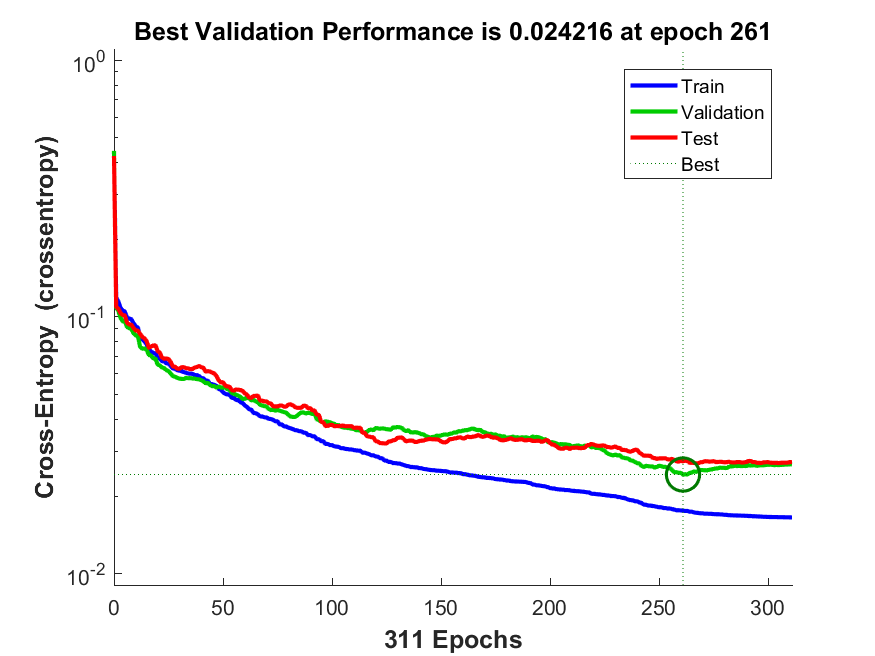
\includegraphics[width=\textwidth]{traincgb50000101.png}
	\caption{Rendimiento mejor caso \lstinline|traincgb|.}
\end{figure}

\newpage

Mejor caso para el algoritmo \lstinline|traincgf|:

\begin{itemize}[noitemsep]
	\item \lstinline|max_fail|: 100.
	\item \lstinline|alpha|: 0.002.
	\item \lstinline|beta|: 0.1.
\end{itemize}

Su gráfico de rendimiento fue:

\begin{figure}[!ht]
	\centering
	\label{fig:traincgb}
	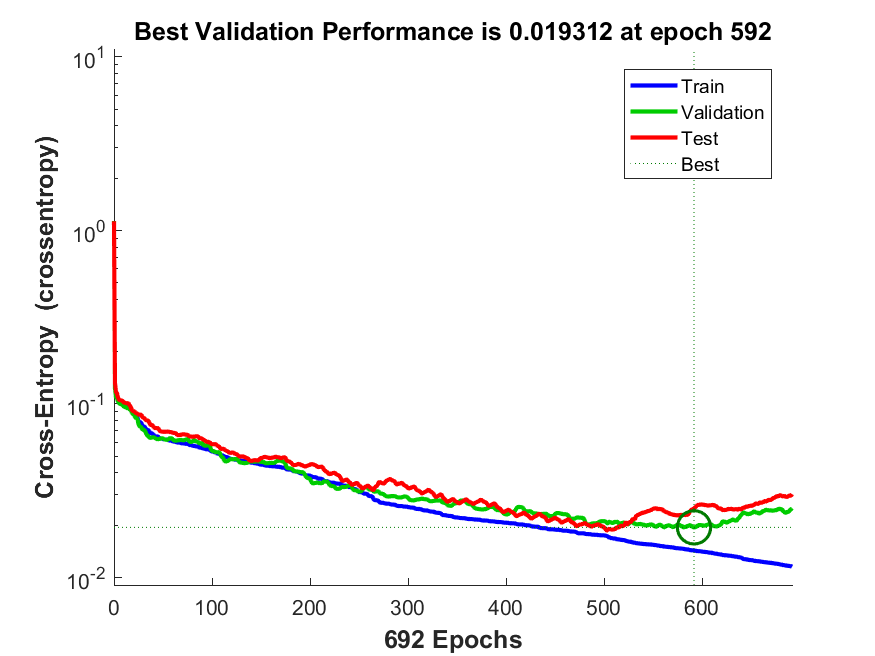
\includegraphics[width=\textwidth]{traincgf10000201.png}
	\caption{Rendimiento mejor caso \lstinline|traincgf|.}
\end{figure}

Hemos observado que los valores \lstinline|alpha| y \lstinline|beta| no afectan en la medida que afecta \lstinline|max_fail|. Por esto, nos hemos limitado a graficar este último parámetro.

\begin{tikzpicture}[every plot/.append style={semithick}]
\begin{axis}[
    xlabel={Max. fail},
    ylabel={Valor de confusión},
    legend pos=south east,
    ymajorgrids=true,
    grid style=dashed,
    scaled ticks=false, % prevent scale labels
    tick label style={/pgf/number format/fixed, % label number format
                      /pgf/number format/precision=3}, 
    width=14cm,
]

\addplot
    coordinates {
(10,0.035986)(20,0.025701)(30,0.024410)(40,0.022194)(50,0.020063)(60,0.020250)(70,0.049056)(80,0.047896)(90,0.043236)(100,0.045826)
    };
    \addlegendentry{traincgb}

\addplot
    coordinates {
    (10,0.048200)(20,0.038600)(30,0.029900)(40,0.026400)(50,0.028500)(60,0.027000)(70,0.025700)(80,0.022300)(90,0.022100)(100,0.019700)
    };
    \addlegendentry{traincgf}
                         
\end{axis}
\end{tikzpicture}

Como podemos observar el algoritmo \lstinline|traincgb| alcalza sus valores mínimos en torno a 50 y luego se dispara. En cambio, el valor de confusión con el algoritmo \lstinline|traincgf| tiende a cero según se incrementa el parámetro \lstinline|max_fail|. 

Para comprobar la tendencia decreciente del segundo algoritmo, hemos realizado otra prueba incrementando el límite superior del parámetro \lstinline|max_fail| a 10.000. De manera que el criterio de parada es el número de \textit{epochs} (1000). El mejor caso obtenido es:

\begin{itemize}[noitemsep]
	\item \lstinline|max_fail|: 10.000.
	\item \lstinline|alpha|: 0.004.
	\item \lstinline|beta|: 0.5.
\end{itemize}

\newpage

Su gráfico de rendimiento fue:

\begin{figure}[!ht]
	\centering
	\label{fig:traincgb}
	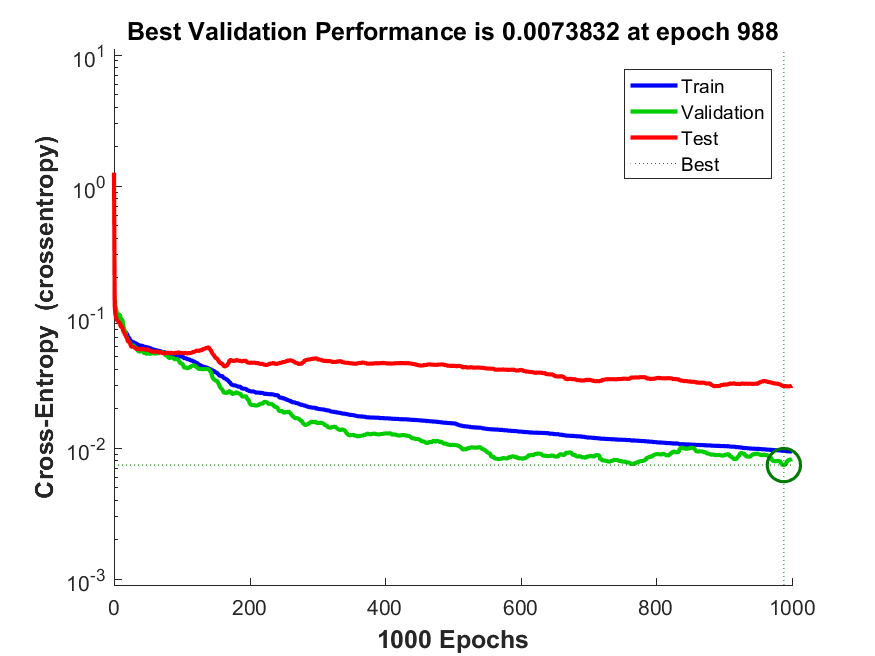
\includegraphics[width=\textwidth]{traincgf560000405.png}
	\caption{Rendimiento mejor caso \lstinline|traincgf|.}
\end{figure}

Vemos como se ha reducido el error hasta un ~0,7\%. Lo cual es una gran mejora respecto a los resultados obtenidos en la primera práctica que estaban en torno al 4,5\% o el 2\% obtenido en el primer experimento de este estudio. 

*El experimento se ha repetido 20 veces para descartar que este buen rendimiento obtenido fuese cosa del azar.

\newpage
\section{Conclusiones}

Tras el análisis de los datos obtenidos, podemos concluir que:

\begin{enumerate}[noitemsep]
	\item El límite de \textit{epochs} por defecto (1.000) es un límite suficientemente alto como no influir en el entrenamiento.
	\item El límite de la función de rendimiento por defecto es 0, lo cual significa que 			hasta que la red neuronal no sea perfecta, esta no va a parar de entrenar. Obviamente, según se aumenta este parámetro los resultados van a empeorar (aunque mejorará el tiempo de entrenamiento).
	\item El tiempo de aprendizaje por defecto es infinito. En nuestro caso, hasta 8 segundos no empezaría a afectar al entrenamiento, y obviamente, cuanto más se reduzca peor entrenada estará la red.
	\item En nuestro caso, con los \textit{learning rates} (para el bias y los pesos) estudiados, no hemos encontrado variación significativa. En pruebas posteriores, se ha visto que estos producían variaciones significativas entre órdenes de magnitud diferentes. Cuanto más altos eran, más rápido era el entrenamiento, pero más varianza había en el entrenamiento de la red.
	\item El único criterio de parada que realmente detenía el entrenamiento en nuestro problema era el parámetro \lstinline|max_fail|. Aumentando este y utilizando \lstinline|traincgf| se consiguieron mejorar los resultados notablemente. Sin embargo, el algoritmo \lstinline|traincgb| conseguía su mejor rendimiento entorno a valores de 50, pero empeoraba según se aumentaban más.
\end{enumerate}

% -------------------------------------------------------------
% Bibliography
% -------------------------------------------------------------
\bibliography{citations}
\bibliographystyle{plainnat}

\end{document}
